\documentclass{article}
\usepackage[utf8]{inputenc}

\title{Homework 8\\
    \large{Topological Data Analysis with Persistent Homology}}
\author{Lucas Emanuel Resck Domingues\\    
    Professor: Raphaël Tinarrage\\\\
    {Escola de Matemática Aplicada}\\
    {Fundação Getulio Vargas}}
\date{\today}

% \usepackage{natbib}
\usepackage{graphicx}
\usepackage{amsmath}
\usepackage{amsfonts}
\usepackage{mathtools}
\usepackage{fullpage}

\begin{document}

    \maketitle

    \noindent \textbf{Exercise 48.} \textit{Let $K = {[0], [1], [2], [3], [4], [5], [0, 1], [1, 2], [2, 3], [3, 4], [4, 5], [5, 0]}$ and $L =
    {[0], [1], [2], [0, 1], [1, 2], [2, 0]}$.
    Consider the simplical map $f \colon i \mapsto i \mathrm{\ modulo \ } 3$. Show that
    the induced map $(f_ 1)_\ast$ is zero.}

    \begin{figure}[!h]
        \centering
        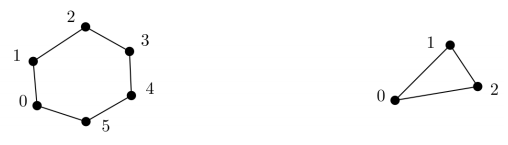
\includegraphics[width=0.6\textwidth]{../figures/exercise_48.png}
    \end{figure}

    There are only two 1-cycles of $K$: $Z_1(K) = \{0, [0, 1] + [1, 2] + [2, 3] + [3, 4] + [4, 5] + [5, 0]\}$.
    Because there are no simplices of dimension 2, the 1-boundary of $K, L$ are $B_1(K) = B_1(L) = \{0\}$.
    So we end up with the two elements of $Z_1(K)$ being the two representants of equivalence classes of $H_1(K) = \{0 + \{0\}, [0, 1] + [1, 2] + [2, 3] + [3, 4] + [4, 5] + [5, 0] + \{0\}\}$.

    Let's applic $(f_1)_\ast$ in our homology group:
    
    \[(f_1)_\ast(0 + B_1(K)) = f_1(0) + B_1(L)= \{0\}\]
    \begin{align*}
            (f_1)_\ast([0, 1] + [1, 2] + [2, 3] + [3, 4] + [4, 5] + [5, 0] + B_1(K)) &= f_1([0, 1] + [1, 2] + [2, 3] + [3, 4] + [4, 5] + [5, 0]) + B_1(L) \\
            &= [0, 1] + [1, 2] + [2, 0] + [0, 1] + [1, 2] + [2, 0] + B_1(K) \\
            &= 0 + B_1(K) \\
            &= \{0\}
    \end{align*}

    We conclude the induced map $(f_1)_\ast$ is zero.

\end{document}
